% use "latex" to generate a *.dvi file, and use "dvisvgm --no-fonts" to convert to .svg
\documentclass[border=10pt]{standalone}
\usepackage{tikz}

\begin{document}

\centering

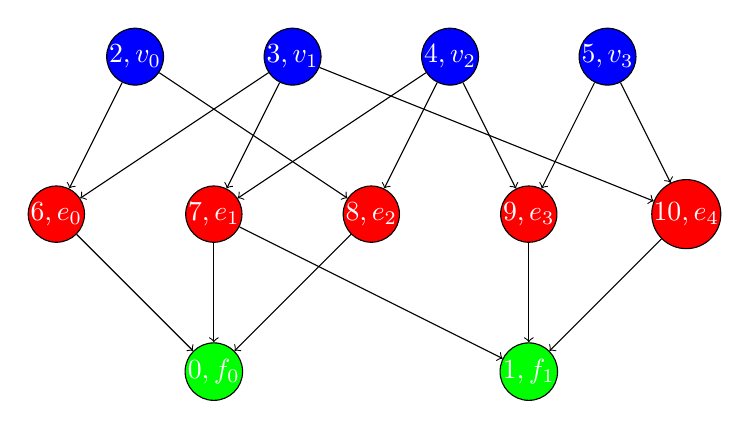
\begin{tikzpicture}[scale=2.0]
  \tikzstyle{vertex}  = [text=blue]
  \tikzstyle{vertexV} = [circle,inner sep=0pt,draw=black,fill=blue,text=white]
  \tikzstyle{edge}    = [text=red]
  \tikzstyle{edgeV}   = [circle,inner sep=0pt,draw=black,fill=red,text=white]
  \tikzstyle{face}    = [text=green]
  \tikzstyle{faceV}   = [circle,inner sep=0pt,draw=black,fill=green,text=white]
  \tikzstyle{sec}     = [->]
  % DAG for doublet
  \path (-1.5, 2.0) node[vertexV](dv0) {$2,v_0$};
  \path (-0.5, 2.0) node[vertexV](dv1) {$3,v_1$};
  \path ( 0.5, 2.0) node[vertexV](dv2) {$4,v_2$};
  \path ( 1.5, 2.0) node[vertexV](dv3) {$5,v_3$};
  \draw (-2.0, 1.0) node[edgeV](e0) {$6,e_0$};
  \draw (-1.0, 1.0) node[edgeV](e1) {$7,e_1$};
  \draw ( 0.0, 1.0) node[edgeV](e2) {$8,e_2$};
  \draw ( 1.0, 1.0) node[edgeV](e3) {$9,e_3$};
  \draw ( 2.0, 1.0) node[edgeV](e4) {$10,e_4$};
  \path (-1.0, 0.0) node[faceV](f0) {$0,f_0$};
  \path ( 1.0, 0.0) node[faceV](f1) {$1,f_1$};
  \draw[sec] (dv0) -- (e0);
  \draw[sec] (dv1) -- (e0);
  \draw[sec] (dv1) -- (e1);
  \draw[sec] (dv2) -- (e1);
  \draw[sec] (dv2) -- (e2);
  \draw[sec] (dv0) -- (e2);
  \draw[sec] (dv2) -- (e3);
  \draw[sec] (dv3) -- (e3);
  \draw[sec] (dv3) -- (e4);
  \draw[sec] (dv1) -- (e4);
  \draw[sec] (e0)  -- (f0);
  \draw[sec] (e1)  -- (f0);
  \draw[sec] (e2)  -- (f0);
  \draw[sec] (e1)  -- (f1);
  \draw[sec] (e3)  -- (f1);
  \draw[sec] (e4)  -- (f1);
\end{tikzpicture}

\end{document}
